\begin{figure}
	\centering
	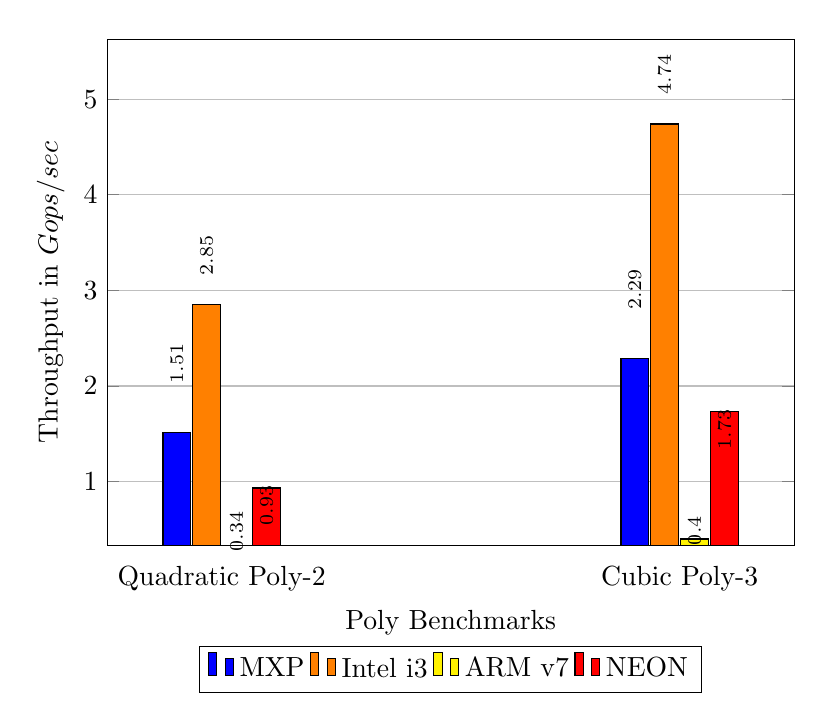
\begin{tikzpicture}
	\begin{axis}[
 	width  = 0.85*\textwidth,
	height = 8cm,
	major x tick style = transparent,
	bar width=10pt,
	ymajorgrids = true,
	ylabel = {Throughput in $Gops/sec$},
	xlabel = {Poly Benchmarks},
	symbolic x coords={Quadratic Poly-2,Cubic Poly-3},
	xtick = data,
	nodes near coords,
	ybar,
	every node near coord/.append style={rotate=90, anchor=west, font=\scriptsize,xshift=0.5cm},
	scaled y ticks = false,
	enlarge y limits={upper,value=0.2},
	enlarge x limits=0.25,
	ybar=2*\pgflinewidth,
	legend cell align=left,
	legend style={
	at={(.5,-0.2)},
	anchor=north,
	legend columns=-1
	column sep=0.5ex
}
	]
	\addplot[draw=black,fill=blue]
	coordinates {(Quadratic Poly-2, 1.5130) (Cubic Poly-3,2.287)};
	
	\addplot[draw=black,fill=orange,every node near coord/.append style={xshift=-0.25cm}]
	coordinates {(Quadratic Poly-2,2.85) (Cubic Poly-3,4.74)};
	
	\addplot[draw=black,fill=yellow,every node near coord/.append style={xshift=-0.70cm}]
	coordinates {(Quadratic Poly-2,0.336) (Cubic Poly-3,0.40)};
	
	\addplot[draw=black,fill=red,every node near coord/.append style={xshift=-1.10cm}]
	coordinates {(Quadratic Poly-2,0.9341) (Cubic Poly-3,1.732)};
	
	\legend{MXP,Intel i3,ARM v7,NEON}
	\end{axis}
	\end{tikzpicture}
	\caption{Byte(8-bits) level throughput(Gops/sec) for polynomial benchmarks }
	\label{poly:1}
\end{figure}